\section{Tips \& Tricks}

\subsection{Daha Hızlı KMeans}
\begin{lstlisting}[language=Python]
# Slow
clf = KMeans(n_clusters=7).fit(X)

# Fast
from sklearn.random_projection import SparseRandomProjection
srp = SparseRandomProjection(n_components=6)
X_srp = srp(X)
clf = KMeans(n_clusters=7).fit(X_srp)
\end{lstlisting}

\subsection{join vs iteration}
Join fonksiyonu iterasyonla eklemeden (sentence += word) daha hızlı çalışır.

\subsection{Activation Function Layer vs Parameter}
Aktivasyon fonksiyonunu katman olarak eklemek parametre olarak eklemekten daha hızlı çalışır.

\subsection{Matplotlib - Subplot Mosaic}
subplots() fonksiyonu eşit boyutlarda grafikler oluştururken, subplot\_mosaic() fonksiyonu farklı ölçeklerde grafikleri tek bir figürde göstermeyi sağlar.

\begin{lstlisting}[language=Python]
ax = fig.subplot_mosaic("""AAB
                           CCC
                           DEF""")

ax["A"].plot()
ax["B"].scatter()
ax["C"].bar()
ax["D"].pie()
ax["E].bar()
ax["F"].plot()
\end{lstlisting}

\subsection{Dont use time.time()}
Model süresini hesaplarken time.time() kullanma. Time.time() güncel zamanı hesaplar. Bunun yerine time.perf\_counter() kullan.

\subsection{DeOldify - Video/Resim Renklendirme}
Siyah-beyaz görüntü/videoları renkli hale getirmek için kullanılan önceden eğitilmiş bir modeldir. Modeli websitesinden indirip proje içerisindeki models klasörüne koymak gerekiyor.

\subsubsection{Resim Renklendirme}
\begin{lstlisting}[language=Python]
from deoldify import device
from deoldify.device_id import DeviceId
from deoldify.visualize import get_image_colorizer, show_image_in_notebook
import warnings
warnings.filterwarnings("ignore")
device.set(device=DeviceId.GPU0)

colorizer = get_image_colorizer(artistic=True)
render_factor = 35
image_path = colorizer.get_platformed_image(path="/path/to/image", render_factor=render_factor, compare=False)
show_image_in_notebook(image_path)
\end{lstlisting}

\subsubsection{Video Renklendirme}
\begin{lstlisting}[language=Python]
from deoldify import device
from deoldify.device_id import DeviceId
from deoldify.visualize import get_video_colorizer, show_video_in_notebook
import warnings
warnings.filterwarnings("ignore")
device.set(device=DeviceId.GPU0)

colorizer = get_video_colorizer()
render_factor = 35
video_path = colorizer.colorizer.colorize_from_file_name(path="/path/to/video", render_factor=render_factor)
show_video_in_notebook(video_path)
\end{lstlisting}

\subsection{Transformer Benchmark}
\begin{lstlisting}[language=Python]
from transformers import PyTorchBenchmark, PyTorchBenchmarkArguments

models = ["bert-base-turkish-uncased", "roberta-base", "albert-base-v2"]

batch_sizes = [4]
sequence_lengths = [64, 128, 256]

args = PyTorchBenchmarkArguments(models=models,
                                 batch_sizes=batch_sizes,
                                 sequence_lengths=sequence_lengths)

benchmark = PyTorchBenchmark(args)
results = benchmark.run()
\end{lstlisting}

\subsection{Stable Diffusion}

\subsubsection{Default Image Generation}
\begin{lstlisting}[language=Python]
import torch
from diffusers import StableDiffusionPipeline

pipeline = StableDiffusionPipeline.from_pretrained(
        "runwayml/stable-diffusion-v1-5",
        torch_dtype = torch.float16
).to("cuda:0")

prompt = ""
image = pipeline(prompt=prompt).images[0]
image
\end{lstlisting}

\subsubsection{Image Generation with Scheduler}
\begin{lstlisting}[language=Python]
import torch
from diffusers import StableDiffusionPipeline, EulerDiscreteScheduler

generator = torch.Generator("cuda:0").manual_seed(42)
pipeline = StableDiffusionPipeline.from_pretrained(
        "runwayml/stable-diffusion-v1-5",
        torch_dtype = torch.float16
)

pipeline.scheduler = EulerDiscreteScheduler.from_config(pipeline.scheduler.config)

prompt = ""
image = pipeline(prompt=prompt,
                 generator=generator,
                 num_inference_steps=30,
                 guidance_scale=10,
                 width=1920,
                 height=1080).images[0]
image
\end{lstlisting}

\subsubsection{Image Generation with Mask}
\begin{lstlisting}[language=Python]
import torch
import cv2
from PIL import Image
from diffusers import StableDiffusionPipeline, EulerDiscreteScheduler

mask_image_path = "mask.png"
mask_data = cv2.imread(mask_file_path)
gray_image = cv2.cvtColor(mask_data, cv2.COLOR_BGR2GRAY)
thresh, mask_image = cv2.threshold(gray_image, 100, 255, cv2.THRESH_BINARY)
mask_image = Image.fromarray(mask_image)

generator = torch.Generator("cuda:0").manual_seed(42)
pipeline = StableDiffusionPipeline.from_pretrained(
        "runwayml/stable-diffusion-v1-5",
        torch_dtype = torch.float16
)

pipeline.scheduler = EulerDiscreteScheduler.from_config(pipeline.scheduler.config)

prompt = ""
image = pipeline(prompt=prompt,
                 generator=generator,
                 num_inference_steps=30,
                 guidance_scale=10,
                 mask_image=mask_image
                 width=1920,
                 height=1080).images[0]
image
\end{lstlisting}

\subsubsection{Super Resolution}
\begin{lstlisting}
import torch
from diffusers import StableDiffusionImg2ImgPipeline

pipeline = StableDiffusionImg2ImgPipeline.from_pretrained(
        "stablediffusionapi/deliberate-v2",
        torch_dtype = torch.float16
).to("cuda:0")

prompt = ""
negative_prompt = ""

image = pipeline(
        image = "path/to/image",
        prompt = prompt,
        negative_prompt = negative_prompt,
        strength = 3,
        num_inference_steps = 100,
        guidance_scale = 7,
        generator = torch.Generator("cuda").manual_seed(42)
).images[0]
image
\end{lstlisting}

\subsection{Prettymaps - Harita Olusturma}
\begin{lstlisting}[language=Python]
import prettymaps
plot = prettymaps.plot(
    'Istanbul Sabahattin Zaim University',
    preset = 'heerhugowaard',
    figsize=(10, 10),
    save_as='image.png'
)
\end{lstlisting}

\begin{figure}[ht]
    \centering
    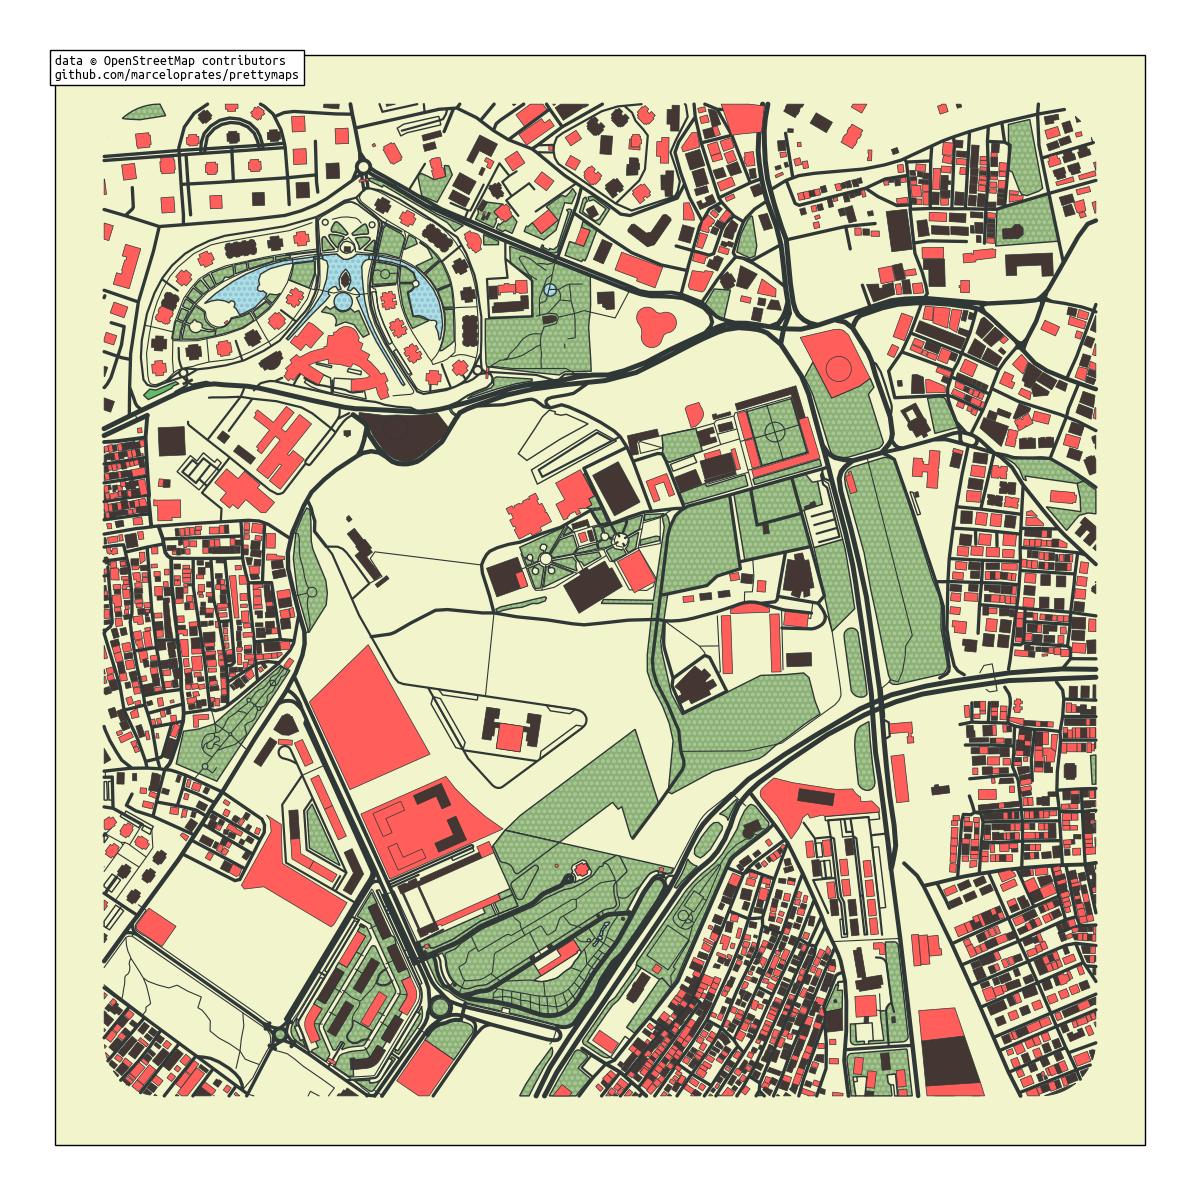
\includegraphics[width=0.5\textwidth]{images/izu.png}
    \caption{Prettymaps IZU.}
    \label{fig:enter-label}
\end{figure}

\newpage

\subsection{Scikeras - Keras HP Tuning}
\begin{lstlisting}[language=Python]
import tensorflow as tf
from scikeras.wrappers import KerasClassifier
from sklearn.model_selection import GridSearchCV

def create_model(units=16, lr_rate=0.1):
    model = tf.keras.Sequential()
    model.add(tf.keras.layers.Dense(units, activation='relu'))
    model.add(tf.keras.layers.Dense(num_classes, activation='softmax'))
    model.compile(optimizer=tf.keras.optimizers.Adam(learning_rate=lr_rate),
                  loss='categorical_crossentropy',
                  metrics=['accuracy'])
    return model

units = [16, 32]
lr_rate = [0.1,0.001]
batch_size = [128, 64]

keras_model = KerasClassifier(build_fn=create_model, 
                              units=units, 
                              lr_rate=lr_rate, 
                              epochs=10, 
                              batch_size=batch_size, 
                              callbacks=[EarlyStopping(monitor='val_loss', patience=3)], 
                              verbose=0)

param_grid = dict(units = units, lr_rate = lr_rate, batch_size = batch_size)
grid = GridSearchCV(estimator = keras_model, param_grid = param_grid, cv = 3)
grid_result = grid.fit(train_data, train_labels)
print("The best parameters are:",grid_result.best_params_)
best_params = grid_result.best_params_
\end{lstlisting}

\subsection{pyLDAvis - Topic Modeling with LDA}
\begin{lstlisting}[language=Python]
import gensim
import pyLDAvis.gensim

tokenized = df["Lemmatization"]
tokenized = [token.split(" ") for token in tokenized]
dictionary = corpora.Dictionary(tokenized)
dictionary.filter_extremes(no_below=1, no_above=0.8)
corpus = [dictionary.doc2bow(tokens) for tokens in tokenized]

ldamodel = gensim.models.ldamodel.LdaModel(corpus, num_topics = 8, id2word=dictionary, passes=15)
lda_display = pyLDAvis.gensim.prepare(ldamodel, corpus, dictionary, sort_topics=True)
pyLDAvis.display(lda_display)
\end{lstlisting}

\subsection{visualkeras - 3D Model Visualization}
\begin{lstlisting}[language=Python]
import tensorflow as tf
import visualkeras

model = tf.keras.Sequential()
model.add(tf.keras.layers.Conv2D(32, (3, 3), activation='relu', input_shape=(224, 224, 3)))
model.add(tf.keras.layers.MaxPooling2D((2, 2)))
model.add(tf.keras.layers.Conv2D(64, (3, 3), activation='relu'))
model.add(tf.keras.layers.MaxPooling2D((2, 2)))
model.add(tf.keras.layers.Conv2D(64, (3, 3), activation='relu'))
model.add(tf.keras.layers.Flatten())
model.add(tf.keras.layers.Dense(32, activation='relu'))
model.add(tf.keras.layers.Dense(10, activation='softmax'))
model.compile(optimizer=tf.keras.optimizers.Adam(),
              loss='categorical_crossentropy',
              metrics=['accuracy'])

visualkeras.layered_view(model, to_file="visualkeras.png").show()
\end{lstlisting}

\begin{figure}[ht]
    \centering
    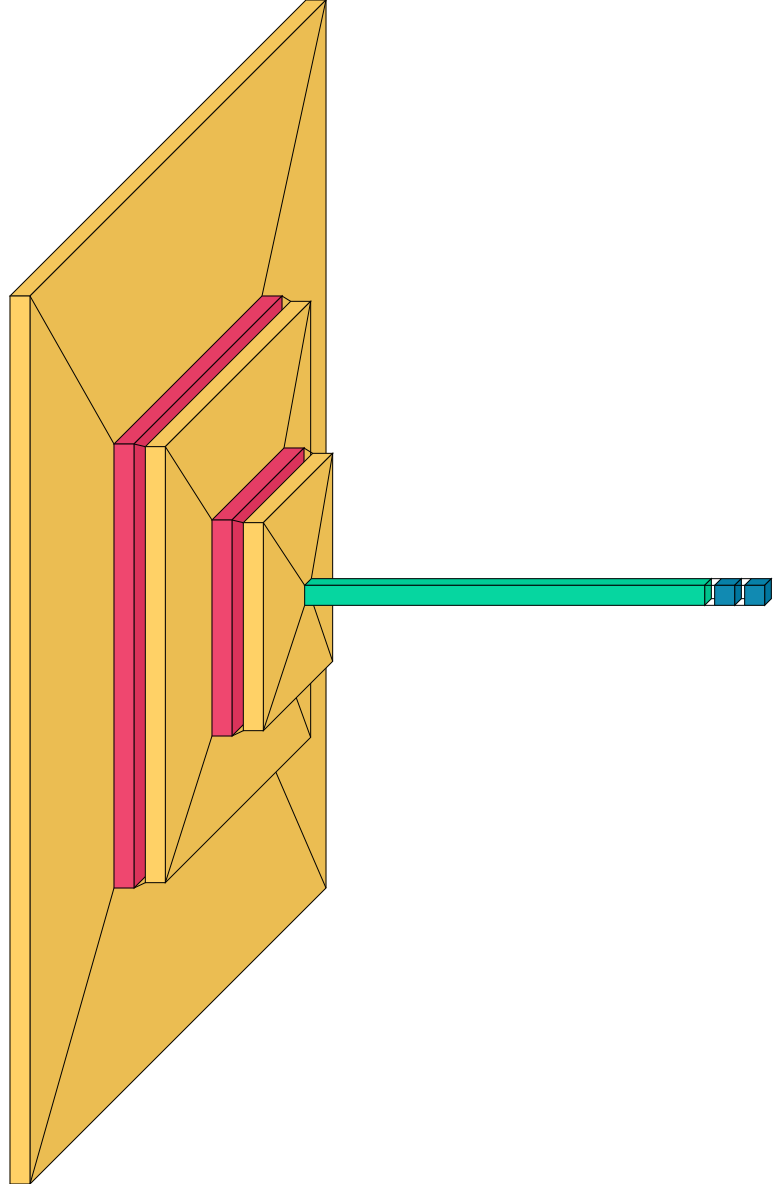
\includegraphics[width=0.25\textwidth]{images/visualkeras.png}
    \caption{visualkeras .}
    \label{fig:enter-label}
\end{figure}

\newpage

\subsection{Plotting N-Grams}
\begin{lstlisting}[language=Python]
def count_ngrams(corpus, ngram, n):
    vec = CountVectorizer(ngram_range=(ngram,ngram)).fit(corpus)
    bag_of_words = vec.transform(corpus)
    sum_words = bag_of_words.sum(axis=0)
    words_freq = [(word, sum_words[0, idx]) for word, idx in vec.vocabulary_.items()]
    words_freq =sorted(words_freq, key = lambda x: x[1], reverse=True)
    return words_freq[:n]
    
def plot_ngrams(ngram_df, ngram_name):
    plt.figure(figsize=(12, 6))
    plt.bar(data=ngram_df, x="Tweets", height="Count")
    plt.xticks(rotation=90)
    plt.xlabel(ngram_name)
    plt.ylabel("Count")
    plt.title(ngram_name)
    plt.show()
    
unigrams = count_ngrams(corpus=df["Lemmatization"], ngram=1, n=30)
top_unigram = pd.DataFrame(unigrams, columns=['Tweets', "Count"])
plot_ngrams(top_unigram, "Unigrams")
\end{lstlisting}

\begin{figure}[ht]
    \centering
    \includegraphics[width=1.0\textwidth]{images/nlp_unigram.png}
    \caption{Unigrams .}
    \label{fig:enter-label}
\end{figure}

\newpage
